\section{РМК}
\subsection{Объекты тестирования, описанные в разделе}

Тестирование рабочего места кассира нужно проводить на кассе и только при подключенном оборудовании ( фискальные регистратор, сканер штрихкодов, весы, табло покупателя)
\begin{longtable}{p{0.05\linewidth}p{0.4\linewidth}p{0.4\linewidth}}
    %  \toprule
    \hline
    1 & Вид объекта & Обработка \\
    \hline
    %     \hline
    %    \endhead
    & Имя & РМКУправляемыйРежим \\
    \hline
    & Синоним  & РМК (управляемый режим) \\
    \hline


    \bottomrule %%% верхняя линейка
\end{longtable}

\newpage
\subsection{РМК (управляемый режим)}
\renewcommand{\arraystretch}{1.8} %% расстояние между строками таблицы
%\begin{landscape}
\begin{longtable}{|p{0.02\linewidth}|p{0.3\linewidth}|p{0.3\linewidth}|p{0.3\linewidth}|}
    %  {|c|c|l|c|}
    \hline
    № & \textbf{Действие} & \textbf{Ожидаемый результат} & \textbf{Фактический результат} \\
    %****************************************************************************************************
    \hline
    \hline
    \endhead
    \multicolumn{4}{|c|}{\textbf{\textit{Проверка запуска РМК при старте}}} \\
    \hline
    \Rownum & Запустить конфигурацию магазина  & 1.Открылся общий интерфейс программы;\par
    2. Отображаются все доступные разделы  &  \\
    \hline
    \Rownum & Перейти в раздел <<Администрирование>>   & 1. Открылся отдел <<Администрирование>>
    &  \\

    \hline
    \Rownum	& Выбрать пункт <<Настройки пользователей и прав>>  & Открылся раздел <<Настройки пользователей и прав>>   &  \\
    \hline
    \Rownum	& Выбрать пункт  <<Пользователи>> & Открылся раздел <<Пользователи>> &  \\
    \hline
    \Rownum & В списке пользователей открыть пользователя с именем  <<Абрамовская Екатерина>> & Открылась форма элемента справочника  <<Пользователи>> со значением <<Абрамовская Екатерина>> &  \\
    \hline
    \Rownum	& Перейти в редактирование закладки <<Группы>> & 1. Открылся список групп, в которые включен пользователь;\par
    2. В списке выбранна группа <<Кассиры>>  &  \\
    \hline
    \Rownum	& Снять выбор с группы <<Кассиры>> и установить выбор на группу <<Заведующие магазинами>>  & Снят выбор с группы <<Кассиры>> и установлен выбор на группу <<Заведующие магазинами>>  &  \\
    \hline
    \Rownum	& Нажать кнопку \keys{Записать}  & Изменения сохранились &  \\
    \hline
    \Rownum	& Перейти в редактирование закладки <<Основное>>  & Открылась форма с основными настройками пользователя  &  \\
    \hline
    \Rownum	& Нажать кнопку \keys{Записать и закрыть} & Закрылась форма элемента справочника  <<Пользователи>> со значением <<Абрамовская Екатерина>>  &  \\
    \hline
    \Rownum	& Закрыть конфигурацию  & Конфигурация закрылась  &  \\
    \hline
    \Rownum & Запустить конфигурацию магазина выбрав пользователя <<Абрамовская Е. (кассир)>> & 1.Открылся общий интерфейс программы;\par
    2. Отображаются все доступные разделы;\par
    3. Обработка <<Рабочее место кассира>> не открылась &  \\
    \hline
     \hline
    \Rownum & Перейти в раздел <<Администрирование>>   & 1. Открылся отдел <<Администрирование>>
    &  \\

    \hline
    \Rownum	& Выбрать пункт <<Настройки пользователей и прав>>  & Открылся раздел <<Настройки пользователей и прав>>   &  \\
    \hline
    \Rownum	& Выбрать пункт  <<Пользователи>> & Открылся раздел <<Пользователи>> &  \\
    \hline
    \Rownum & В списке пользователей открыть пользователя с именем  <<Абрамовская Екатерина>> & Открылась форма элемента справочника  <<Пользователи>> со значением <<Абрамовская Екатерина>> &  \\
    \hline
    \Rownum	& Перейти в редактирование закладки <<Группы>> & 1. Открылся список групп, в которые включен пользователь;\par
    2. В списке выбранна группа <<Заведующие магазинами>>  &  \\
    \hline
    \Rownum	& Снять выбор с группы <<Заведующие магазинами>> и установить выбор на группу <<Кассиры>>  & Снят выбор с группы <<Заведующие магазинами>> и установлен выбор на группу <<Кассиры>>  &  \\
    \hline
    \Rownum	& Нажать кнопку \keys{Записать}  & Изменения сохранились &  \\
    \hline
    \Rownum	& Перейти в редактирование закладки <<Основное>>  & Открылась форма с основными настройками пользователя  &  \\
    \hline

    \Rownum	& Нажать кнопку \keys{Записать и закрыть} & Закрылась форма элемента справочника  <<Пользователи>> со значением <<Абрамовская Екатерина>>  &  \\
    \hline
    \Rownum	& Закрыть конфигурацию  & Конфигурация закрылась  &  \\
    \hline
    \Rownum & Запустить конфигурацию магазина выбрав пользователя <<Абрамовская Е. (кассир)>> & 1.Открылся общий интерфейс программы;\par
    2. Отображаются разделы <<Главное>> и <<Продажи>>;\par
    3. Открылась обработка <<Рабочее место кассира>>  &  \\
    \hline
    %****************************************************************************************************



    %****************************************************************************************************

    \multicolumn{4}{|c|}{\textbf{\textit{Проверка возможности открытия кассовой смены}}} \\
    \hline
     \hline
    \Rownum & Запустить конфигурацию магазина выбрав пользователя <<Абрамовская Е. (кассир)>> & 1.Открылся общий интерфейс программы;\par
    2. Отображаются разделы <<Главное>> и <<Продажи>>;\par
    3. Открылась обработка <<Рабочее место кассира>>  &  \\
    \hline
    \Rownum	& Нажать кнопку \keys{Открытие смены} в меню РМК & 1. Кассовая смена открыта;\par
    2. На фискальном регистраторе напечатан чек открытия смены &  \\
    \hline
    %****************************************************************************************************



    \multicolumn{4}{|c|}{\textbf{\textit{Изменена основная форма РМК, уменьшен размер}}} \\
    \hline
    \hline
    \Rownum & Запустить конфигурацию магазина выбрав пользователя <<Абрамовская Е. (кассир)>> & 1.Открылся общий интерфейс программы;\par
    2. Отображаются разделы <<Главное>> и <<Продажи>>;\par
    3. Открылась обработка <<Рабочее место кассира>>  &  \\

    \hline
    \Rownum	& Нажать кнопку \keys{Регистрация продаж} в меню РМК & 1. Форма меню РМК закрыта;\par
    2. Открыта форма с информационным сообщением для кассиров;\par
    3. Кнопка \keys{ОК} в нижней части формы недоступна &  \\
    \hline
    \Rownum	& Отметить чек бокс с надписью <<Мною прочитано и понято>> & 1. Чек бокс с надписью <<Мною прочитано и понято>> отмечен ;\par
    2. Кнопка \keys{ОК} в нижней части формы доступна &   \\
    \hline
    \Rownum	& Нажать кнопку \keys{ОК} в нижней части формы & 1. Форма с информационным сообщением для кассиров закрыта.;\par
    2. Открыта форма Рабочего места кассира;\par
    3. Форма имеет корректные размеры и вмещается на экран без вертикальных и горизонтальных полос прокрутки  &  \\
    \hline
    \Rownum & Закрыть рабочее место кассира нажав последовательно горячие клавиши \keys{F10} - \keys{F12}  & Открылось меню <<Рабочего места кассира>>;\par
     &  \\
    \hline
    \Rownum & Нажать кнопку \keys{Завершение работы}   & Конфигурация закрылась
    &  \\
    \hline
    %****************************************************************************************************

    \multicolumn{4}{|c|}{\textbf{\textit{Проверка различных алгоритмов и элементов формы}}} \\
    \hline
    \hline
    \Rownum & Запустить конфигурацию магазина выбрав пользователя <<Абрамовская Е. (кассир)>> & 1.Открылся общий интерфейс программы;\par
    2. Отображаются разделы <<Главное>> и <<Продажи>>;\par
    3. Открылась обработка <<Рабочее место кассира>>  &  \\
    \hline
    \Rownum	& Нажать кнопку \keys{Регистрация продаж} в меню РМК & 1. Форма меню РМК закрыта;\par
    2. Открыта форма с информационным сообщением для кассиров;\par
    3. Кнопка \keys{ОК} в нижней части формы недоступна &  \\
    \hline
    \Rownum	& Отметить чек бокс с надписью <<Мною прочитано и понято>> & 1. Чек бокс с надписью <<Мною прочитано и понято>> отмечен ;\par
    2. Кнопка \keys{ОК} в нижней части формы доступна &   \\
    \hline
    \Rownum	& Нажать кнопку \keys{ОК} в нижней части формы & 1. Форма с информационным сообщением для кассиров закрыта.;\par
    2. Открыта форма Рабочего места кассира  &  \\
    \hline
    \Rownum	& Проверить кнопки в верхней части формы & Присутствуют кнопки:\par 1. <<Меню>>;\par
    2. <<Поиск>>;\par
    3. <<Ред.строки>>;\par
    4. <<Возврат>>;\par
    5. <<Бонусы>>;\par
    6. <<Оплата>>;\par
    7. <<Проверить чеки ККМ>> &  \\
    \hline
     \Rownum	& Проверить наличие надписи <<ОстатокБонусов>> & 1. Присутствует надпись <<Остаток бонусов на карте>>;\par
    2. Справа от надписи поле ввода со значением <<0>>;\par
    3. Справа от поля ввода кнопка <<Обновить состояния дисконтного сервера>> &  \\
    \hline
    \Rownum	& Проверить состав полей в табличной части <<Товары>> & Присутствуют только поля:\par
    1. <<Артикул>>;\par
    2. <<Номенклатура>>;\par
    3. <<Количество>>;\par
    4. <<Цена>>;\par
    5. <<Сумма>> &  \\
    \hline
    \Rownum	& Нажать кнопку \keys{Поиск (F11)} в верхней части формы или горячую клавишу \keys{F11} & Открыта форма поиска и подбора товара в РМК &  \\
    \hline
    \Rownum	& Нажать на текстовую метку <<Показать информацию>> в нижней части формы  & 1. В нижней части формы отображается табличная часть;\par
    2. Под табличной частью чек бокс <<остатки>> недоступен для редактирования &  \\
    \hline
    %****************************************************************************************************

     \multicolumn{4}{|c|}{\textbf{\textit{Проверка автоматического подбора количества разливного пива при выборе тары}}} \\
    \hline
    \hline
    \Rownum & Запустить конфигурацию магазина выбрав пользователя <<Абрамовская Е. (кассир)>> & 1.Открылся общий интерфейс программы;\par
    2. Отображаются разделы <<Главное>> и <<Продажи>>;\par
    3. Открылась обработка <<Рабочее место кассира>>  &  \\
    \hline
    \Rownum	& Нажать кнопку \keys{Регистрация продаж} в меню РМК & 1. Форма меню РМК закрыта;\par
    2. Открыта форма с информационным сообщением для кассиров;\par
    3. Кнопка \keys{ОК} в нижней части формы недоступна &  \\
    \hline
    \Rownum	& Отметить чек бокс с надписью <<Мною прочитано и понято>> & 1. Чек бокс с надписью <<Мною прочитано и понято>> отмечен ;\par
    2. Кнопка \keys{ОК} в нижней части формы доступна &   \\
    \hline
    \Rownum	& Нажать кнопку \keys{ОК} в нижней части формы & 1. Форма с информационным сообщением для кассиров закрыта.;\par
    2. Открыта форма Рабочего места кассира  &  \\
    \hline
    \Rownum	& Нажать кнопку \keys{Поиск (F11)} в верхней части формы или горячую клавишу \keys{F11} & Открыта форма поиска и подбора товара в РМК &  \\
    \hline
    \Rownum	& Выбрать поиск по наименованию в выпадающем списке <<Поиск>> верхней части формы  & Выбран режим поиска по наименованию &  \\
    \hline
    \Rownum	& В поле поиска ввести <<Трое в лодке светлое>>  & В табличной части <<Товары>> осталась номенклатура, в наименовании которой содержится <<Трое в лодке светлое>> &  \\
    \hline
    \Rownum	& В табличной части <<Товары>> выбрать позицию с артикулом <<11697>>  & 1. Форма поиска закрылась;\par
    2. В табличную часть <<Товары>> формы рабочего места кассира добавлена позиция с артикулом <<11697>> с количеством <<1>> и установленной ценой &  \\
    \hline
    \Rownum	& Нажать \keys{Ctrl} + \keys{M}   & 1. В табличную часть <<Товары>> формы рабочего места кассира добавлена позиция с артикулом <<10340>> - <<ПЭТ бутылка 1,5л>>  &  \\
    \hline
    \Rownum	& Установить количество позиции с артикулом <<10340>> равным <<2>>  & 1. Количество позиции с артикулом <<11697>> - <<Пиво Трое в лодке светлое 1л>> изменилось на значение <<3>>&  \\
    \hline
    %****************************************************************************************************


    \multicolumn{4}{|c|}{\textbf{\textit{Проверка запрета продажи разливного товара без тары}}} \\
    \hline
    \hline
    \Rownum & Запустить конфигурацию магазина выбрав пользователя <<Абрамовская Е. (кассир)>> & 1.Открылся общий интерфейс программы;\par
    2. Отображаются разделы <<Главное>> и <<Продажи>>;\par
    3. Открылась обработка <<Рабочее место кассира>>  &  \\
    \hline
    \Rownum	& Нажать кнопку \keys{Регистрация продаж} в меню РМК & 1. Форма меню РМК закрыта;\par
    2. Открыта форма с информационным сообщением для кассиров;\par
    3. Кнопка \keys{ОК} в нижней части формы недоступна &  \\
    \hline
    \Rownum	& Отметить чек бокс с надписью <<Мною прочитано и понято>> & 1. Чек бокс с надписью <<Мною прочитано и понято>> отмечен ;\par
    2. Кнопка \keys{ОК} в нижней части формы доступна &   \\
    \hline
    \Rownum	& Нажать кнопку \keys{ОК} в нижней части формы & 1. Форма с информационным сообщением для кассиров закрыта.;\par
    2. Открыта форма Рабочего места кассира  &  \\
    \hline
    \Rownum	& Нажать кнопку \keys{Поиск (F11)} в верхней части формы или горячую клавишу \keys{F11} & Открыта форма поиска и подбора товара в РМК &  \\
    \hline
    \Rownum	& Выбрать поиск по наименованию в выпадающем списке <<Поиск>> верхней части формы  & Выбран режим поиска по наименованию &  \\
    \hline
    \Rownum	& В поле поиска ввести <<Трое в лодке светлое>>  & В табличной части <<Товары>> осталась номенклатура, в наименовании которой содержится <<Трое в лодке светлое>> &  \\
    \hline
    \Rownum	& В табличной части <<Товары>> выбрать позицию с артикулом <<11697>>  & 1. Форма поиска закрылась;\par
    2. В табличную часть <<Товары>> формы рабочего места кассира добавлена позиция с артикулом <<11697>> с количеством <<1>> и установленной ценой &  \\
    \hline
    \Rownum	& Нажать кнопку \keys{Оплата (F8)} в верхней части формы или горячую клавишу \keys{F8}  & Открыта форма с информационным сообщением << Внимание! Объём тары и объём разливных напитков расходятся на -1л. !>>  &  \\
    \hline

    %****************************************************************************************************


     \multicolumn{4}{|c|}{\textbf{\textit{Проверка сообщения о превышении количества}}} \\
    \hline
    \hline
    \Rownum & Запустить конфигурацию магазина выбрав пользователя <<Абрамовская Е. (кассир)>> & 1.Открылся общий интерфейс программы;\par
    2. Отображаются разделы <<Главное>> и <<Продажи>>;\par
    3. Открылась обработка <<Рабочее место кассира>>  &  \\
    \hline
    \Rownum	& Нажать кнопку \keys{Регистрация продаж} в меню РМК & 1. Форма меню РМК закрыта;\par
    2. Открыта форма с информационным сообщением для кассиров;\par
    3. Кнопка \keys{ОК} в нижней части формы недоступна &  \\
    \hline
    \Rownum	& Отметить чек бокс с надписью <<Мною прочитано и понято>> & 1. Чек бокс с надписью <<Мною прочитано и понято>> отмечен ;\par
    2. Кнопка \keys{ОК} в нижней части формы доступна &   \\
    \hline
    \Rownum	& Нажать кнопку \keys{ОК} в нижней части формы & 1. Форма с информационным сообщением для кассиров закрыта.;\par
    2. Открыта форма Рабочего места кассира  &  \\
    \hline
    \Rownum	& Нажать кнопку \keys{Поиск (F11)} в верхней части формы или горячую клавишу \keys{F11} & Открыта форма поиска и подбора товара в РМК &  \\
    \hline
    \Rownum	& Выбрать поиск по наименованию в выпадающем списке <<Поиск>> верхней части формы  & Выбран режим поиска по наименованию &  \\
    \hline
    \Rownum	& В поле поиска ввести <<Трое в лодке светлое>>  & В табличной части <<Товары>> осталась номенклатура, в наименовании которой содержится <<Трое в лодке светлое>> &  \\
    \hline
    \Rownum	& В табличной части <<Товары>> выбрать позицию с артикулом <<11697>>  & 1. Форма поиска закрылась;\par
    2. В табличную часть <<Товары>> формы рабочего места кассира добавлена позиция с артикулом <<11697>> с количеством <<1>> и установленной ценой &  \\
    \hline

    \Rownum	& Нажать \keys{Ctrl} + \keys{M}   & 1. В табличную часть <<Товары>> формы рабочего места кассира добавлена позиция с артикулом <<10340>> - <<ПЭТ бутылка 1,5л>>  &  \\
    \hline
    \Rownum	& Установить количество позиции с артикулом <<10340>> равным <<20 000>>  & 1. Количество позиции с артикулом <<11697>> - <<Пиво Трое в лодке светлое 1л>> изменилось на значение <<30 000>>&  \\
    \hline
    \Rownum	& Нажать кнопку \keys{Оплата (F8)} в верхней части формы или горячую клавишу \keys{F8}  & 1. Открыта форма с информационным сообщением << Отрицательные остатки  ПЭТ бутылка 1,5л
    Превышен остаток на складе  <<указан склад>>
    Пиво Трое в лодке светлое 1л
    Превышен остаток на складе <<указан склад>> !>>;\par
    2. Количество на сколько превышен остаток не указано  &  \\
    \hline
    %****************************************************************************************************


      \multicolumn{4}{|c|}{\textbf{\textit{Проверка различных алгоритмов и элементов формы оплаты}}} \\
    \hline
    \hline
    \Rownum & Запустить конфигурацию магазина выбрав пользователя <<Абрамовская Е. (кассир)>> & 1.Открылся общий интерфейс программы;\par
    2. Отображаются разделы <<Главное>> и <<Продажи>>;\par
    3. Открылась обработка <<Рабочее место кассира>>  &  \\
    \hline
    \Rownum	& Нажать кнопку \keys{Регистрация продаж} в меню РМК & 1. Форма меню РМК закрыта;\par
    2. Открыта форма с информационным сообщением для кассиров;\par
    3. Кнопка \keys{ОК} в нижней части формы недоступна &  \\
    \hline
    \Rownum	& Отметить чек бокс с надписью <<Мною прочитано и понято>> & 1. Чек бокс с надписью <<Мною прочитано и понято>> отмечен ;\par
    2. Кнопка \keys{ОК} в нижней части формы доступна &   \\
    \hline
    \Rownum	& Нажать кнопку \keys{ОК} в нижней части формы & 1. Форма с информационным сообщением для кассиров закрыта.;\par
    2. Открыта форма Рабочего места кассира  &  \\
    \hline
    \Rownum	& Нажать кнопку \keys{Поиск (F11)} в верхней части формы или горячую клавишу \keys{F11} & Открыта форма поиска и подбора товара в РМК &  \\
    \hline
    \Rownum	& Выбрать поиск по наименованию в выпадающем списке <<Поиск>> верхней части формы  & Выбран режим поиска по наименованию &  \\
    \hline
    \Rownum	& В поле поиска ввести <<Трое в лодке светлое>>  & В табличной части <<Товары>> осталась номенклатура, в наименовании которой содержится <<Трое в лодке светлое>> &  \\
    \hline
    \Rownum	& В табличной части <<Товары>> выбрать позицию с артикулом <<11697>>  & 1. Форма поиска закрылась;\par
    2. В табличную часть <<Товары>> формы рабочего места кассира добавлена позиция с артикулом <<11697>> с количеством <<1>> и установленной ценой &  \\
    \hline

    \Rownum	& Нажать \keys{Ctrl} + \keys{M}   & 1. В табличную часть <<Товары>> формы рабочего места кассира добавлена позиция с артикулом <<10340>> - <<ПЭТ бутылка 1,5л>>  &  \\
    \hline
    \Rownum	& Установить количество позиции с артикулом <<10340>> равным <<1>>  & 1. Количество позиции с артикулом <<11697>> - <<Пиво Трое в лодке светлое 1л>> изменилось на значение <<1.5>>&  \\
    \hline
    \Rownum	& Нажать кнопку \keys{Оплата (F8)} в верхней части формы или горячую клавишу \keys{F8}  & 1. Открыта форма оплаты товара  &  \\
    \hline

    \Rownum& Проверить кнопки справа от поля <<Всего к оплате (руб):>> & Присутствуют только кнопки:\par 1.  <<Нал.(F6)>>;\par
    2. <<ПК(F7)>> &  \\
    \hline

    \Rownum& Проверить кнопки справа от поля <<Остаток (руб):>> & Присутствуют только кнопки:\par 1. <<Послать чек электронным письмом (Ctrl+C)>>;\par
    2. <<Послать чек SMS (Ctrl+S)>> &  \\
    \hline
    %****************************************************************************************************




     \multicolumn{4}{|c|}{\textbf{\textit{Проверка простого чека с алкоголем}}} \\
    \hline
    \hline
    \Rownum & Запустить конфигурацию магазина выбрав пользователя <<Абрамовская Е. (кассир)>> & 1.Открылся общий интерфейс программы;\par
    2. Отображаются разделы <<Главное>> и <<Продажи>>;\par
    3. Открылась обработка <<Рабочее место кассира>>  &  \\
    \hline
    \Rownum	& Нажать кнопку \keys{Регистрация продаж} в меню РМК & 1. Форма меню РМК закрыта;\par
    2. Открыта форма с информационным сообщением для кассиров;\par
    3. Кнопка \keys{ОК} в нижней части формы недоступна &  \\
    \hline
    \Rownum	& Отметить чек бокс с надписью <<Мною прочитано и понято>> & 1. Чек бокс с надписью <<Мною прочитано и понято>> отмечен ;\par
    2. Кнопка \keys{ОК} в нижней части формы доступна &   \\
    \hline
    \Rownum	& Нажать кнопку \keys{ОК} в нижней части формы & 1. Форма с информационным сообщением для кассиров закрыта.;\par
    2. Открыта форма Рабочего места кассира  &  \\
    \hline
    \Rownum	& Нажать кнопку \keys{Поиск (F11)} в верхней части формы или горячую клавишу \keys{F11} & Открыта форма поиска и подбора товара в РМК &  \\
    \hline
    \Rownum	& Выбрать поиск по наименованию в выпадающем списке <<Поиск>> верхней части формы  & Выбран режим поиска по наименованию &  \\
    \hline
    \Rownum	& В поле поиска ввести <<Трое в лодке светлое>>  & В табличной части <<Товары>> осталась номенклатура, в наименовании которой содержится <<Трое в лодке светлое>> &  \\
    \hline
    \Rownum	& В табличной части <<Товары>> выбрать позицию с артикулом <<11697>>  & 1. Форма поиска закрылась;\par
    2. В табличную часть <<Товары>> формы рабочего места кассира добавлена позиция с артикулом <<11697>> с количеством <<1>> и установленной ценой &  \\
    \hline
     \Rownum	& Нажать кнопку \keys{Поиск (F11)} в верхней части формы или горячую клавишу \keys{F11} & Открыта форма поиска и подбора товара в РМК &  \\
    \hline
    \Rownum	& Выбрать поиск по наименованию в выпадающем списке <<Поиск>> верхней части формы  & Выбран режим поиска по наименованию &  \\
    \hline
    \Rownum	& В поле поиска ввести <<Пакет Крюгер Хаус маленький>>  & В табличной части <<Товары>> осталась номенклатура, в наименовании которой содержится <<Пакет Крюгер Хаус маленький>> &  \\
    \hline
    \Rownum	& В табличной части <<Товары>> выбрать позицию с артикулом <<10347>>  & 1. Форма поиска закрылась;\par
    2. В табличную часть <<Товары>> формы рабочего места кассира добавлена позиция с артикулом <<10347>> с количеством <<1>> и установленной ценой &  \\
    \hline
    \Rownum	& Нажать \keys{Ctrl} + \keys{M}   & 1. В табличную часть <<Товары>> формы рабочего места кассира добавлена позиция с артикулом <<10340>> - <<ПЭТ бутылка 1,5л>>  &  \\
    \hline
    \Rownum	& Установить количество позиции с артикулом <<10340>> равным <<1>>  & 1. Количество позиции с артикулом <<11697>> - <<Пиво Трое в лодке светлое 1л>> изменилось на значение <<1.5>>&  \\
    \hline
    \Rownum	& Нажать кнопку \keys{Оплата (F8)} в верхней части формы или горячую клавишу \keys{F8}  &  Открыта форма оплаты &  \\
    \hline
    \Rownum	& Нажать кнопку \keys{Нал.(F6)} справа от поля ввода <<Всего к оплате (руб):>> или горячую клавишу \keys{F6}  & В табличную часть <<Виды оплат>> добавлена строка со значениями полей: <<Вида оплаты>> - <<Наличные>>; <<Сумма>> - рассчитанной суммой&  \\
    \hline
    \Rownum	& Нажать кнопку \keys{Enter} в области цифровых кнопок или горячую клавишу \keys{Ctrl + Enter}  & 1. Форма оплаты закроется;\par
    2. На фискальном регистраторе будет напечатан чек вида:
    \begin{tikzpicture}
        \pgftext{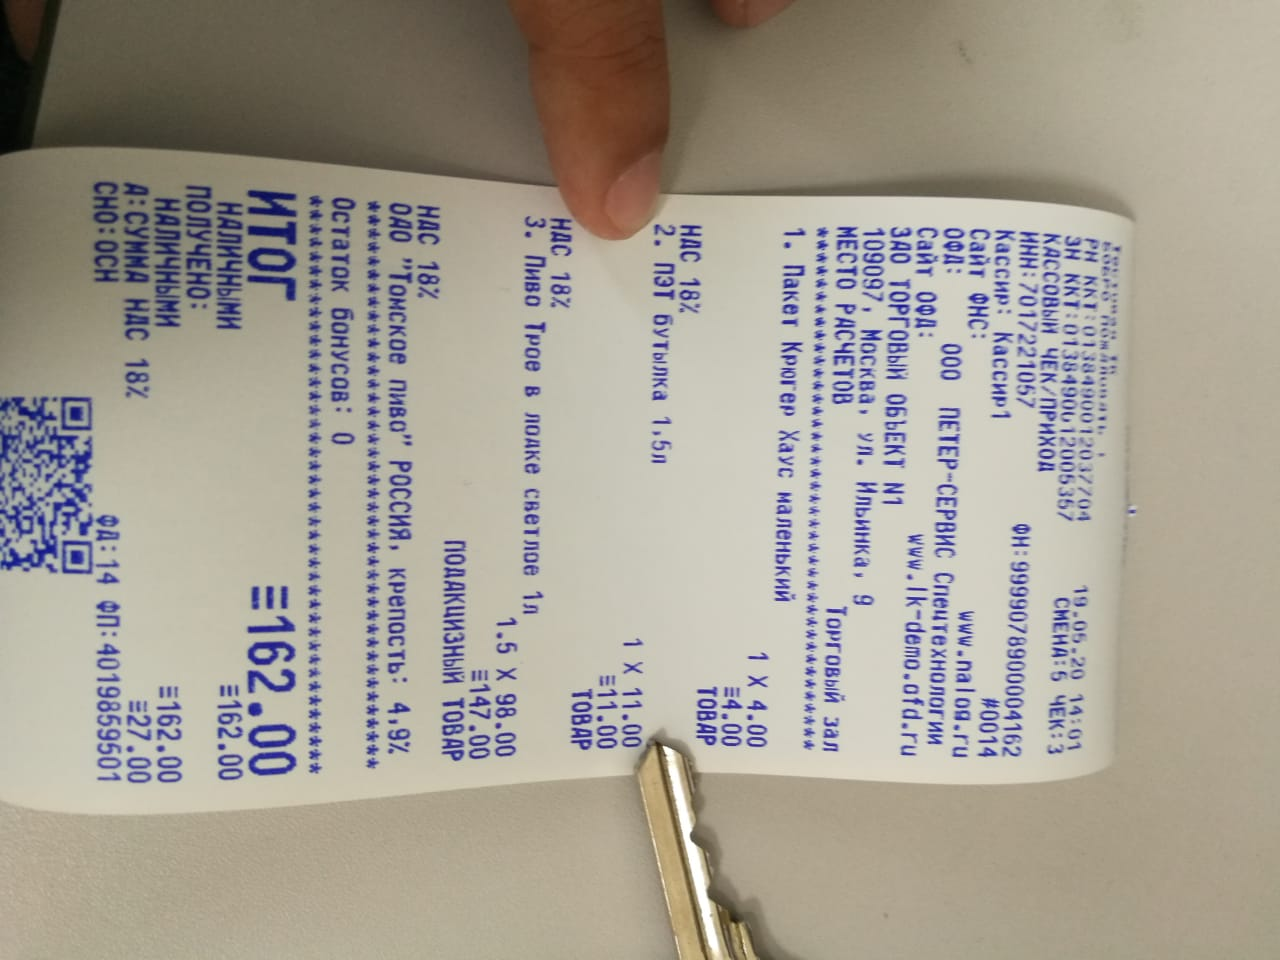
\includegraphics[width=225pt]{2.jpeg}} at (0pt,0pt)
    \end{tikzpicture}
    ;\par
    3. Табличная часть <<Товары>> в форме рабочего места кассира очистится;\par
    4. Поле <<СНО>> в чеке имеет значение <<ОСН>>&  \\
    \hline
    %****************************************************************************************************


   \multicolumn{4}{|c|}{\textbf{\textit{Проверка простого чека с кулинарией}}} \\
   \hline
   \hline
   \Rownum & Запустить конфигурацию магазина выбрав пользователя <<Абрамовская Е. (кассир)>> & 1.Открылся общий интерфейс программы;\par
   2. Отображаются разделы <<Главное>> и <<Продажи>>;\par
   3. Открылась обработка <<Рабочее место кассира>>  &  \\
   \hline
   \Rownum	& Нажать кнопку \keys{Регистрация продаж} в меню РМК & 1. Форма меню РМК закрыта;\par
   2. Открыта форма с информационным сообщением для кассиров;\par
   3. Кнопка \keys{ОК} в нижней части формы недоступна &  \\
   \hline
   \Rownum	& Отметить чек бокс с надписью <<Мною прочитано и понято>> & 1. Чек бокс с надписью <<Мною прочитано и понято>> отмечен ;\par
   2. Кнопка \keys{ОК} в нижней части формы доступна &   \\
   \hline
   \Rownum	& Нажать кнопку \keys{ОК} в нижней части формы & 1. Форма с информационным сообщением для кассиров закрыта.;\par
   2. Открыта форма Рабочего места кассира  &  \\
   \hline
   \Rownum	& Нажать кнопку \keys{Поиск (F11)} в верхней части формы или горячую клавишу \keys{F11} & Открыта форма поиска и подбора товара в РМК &  \\
   \hline
   \Rownum	& Выбрать поиск по наименованию в выпадающем списке <<Поиск>> верхней части формы  & Выбран режим поиска по наименованию &  \\
   \hline
   \Rownum	& В поле поиска ввести <<Гренки чесночные>>  & В табличной части <<Товары>> осталась номенклатура, в наименовании которой содержится <<Гренки чесночные>> &  \\
   \hline
   \Rownum	& В табличной части <<Товары>> выбрать позицию с артикулом <<11432>>  & 1. Форма поиска закрылась;\par
   2. В табличную часть <<Товары>> формы рабочего места кассира добавлена позиция с артикулом <<11432>> с количеством <<1>> и установленной ценой &  \\
   \Rownum	& Установить количество позиции с артикулом <<11432>> равным <<0,150>>  & 1. Количество позиции с артикулом <<11432>> - <<Гренки чесночные>> изменилось на значение <<0,150>>&  \\
   \hline

   \Rownum	& Нажать кнопку \keys{Оплата (F8)} в верхней части формы или горячую клавишу \keys{F8}  &  Открыта форма оплаты &  \\
   \hline
   \Rownum	& Нажать кнопку \keys{Нал.(F6)} справа от поля ввода <<Всего к оплате (руб):>> или горячую клавишу \keys{F6}  & В табличную часть <<Виды оплат>> добавлена строка со значениями полей: <<Вида оплаты>> - <<Наличные>>; <<Сумма>> - рассчитанной суммой&  \\
   \hline
   \Rownum	& Нажать кнопку \keys{Enter} в области цифровых кнопок или горячую клавишу \keys{Ctrl + Enter}  & 1. Форма оплаты закроется;\par
   2. На фискальном регистраторе будет напечатан чек вида:
   \begin{tikzpicture}
   \pgftext{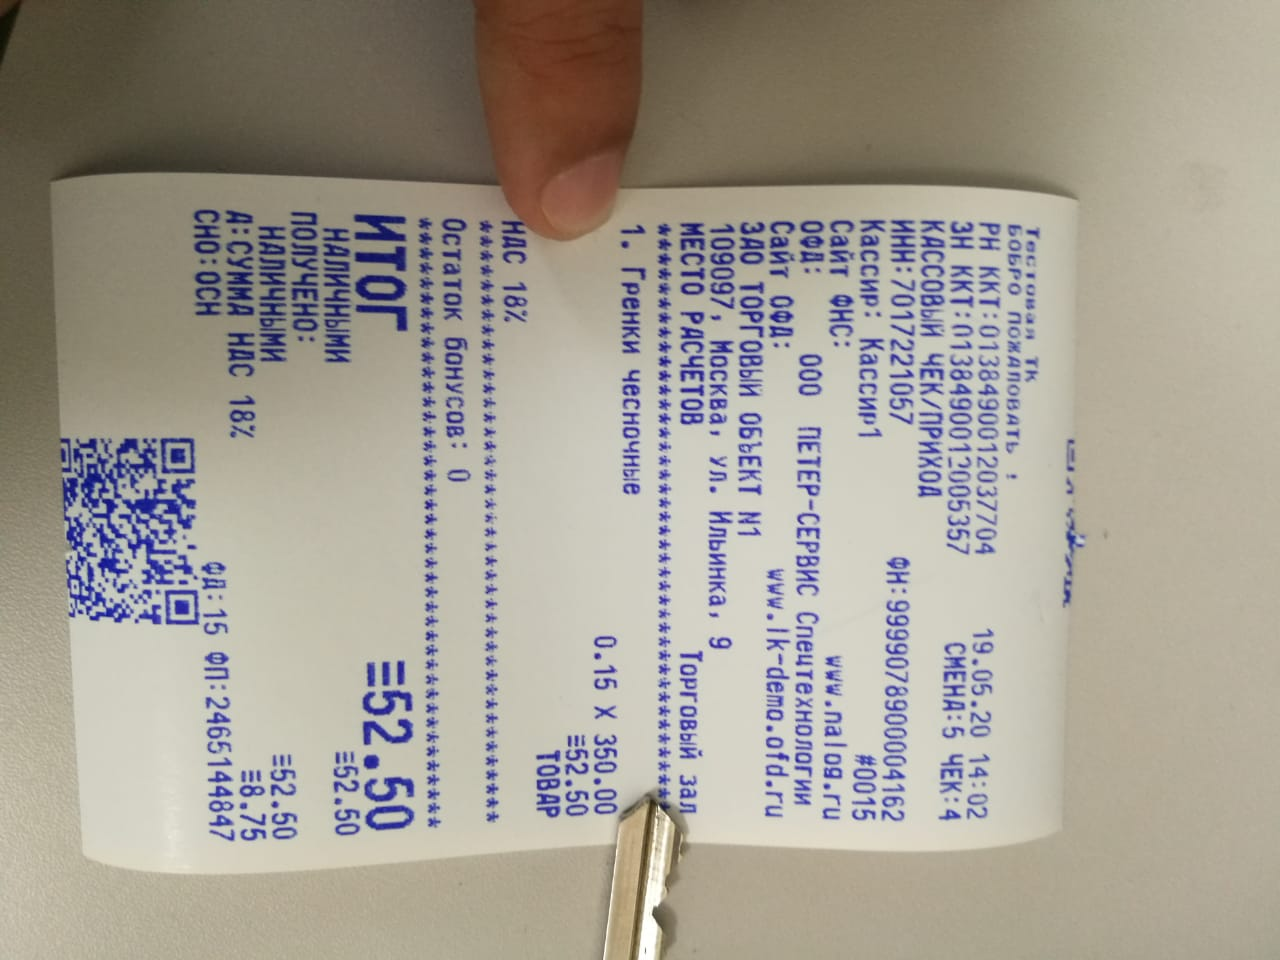
\includegraphics[width=225pt]{3.jpeg}} at (0pt,0pt)
   \end{tikzpicture}
   ;\par
   3. Табличная часть <<Товары>> в форме рабочего места кассира очистится;\par
   4. Поле <<СНО>> в чеке имеет значение <<УСН>>&  \\
   \hline
   %****************************************************************************************************




    \multicolumn{4}{|c|}{\textbf{\textit{Проверка чека с кулинарией и прочим товаром}}} \\
   \hline
   \hline
   \Rownum & Запустить конфигурацию магазина выбрав пользователя <<Абрамовская Е. (кассир)>> & 1.Открылся общий интерфейс программы;\par
   2. Отображаются разделы <<Главное>> и <<Продажи>>;\par
   3. Открылась обработка <<Рабочее место кассира>>  &  \\
   \hline
   \Rownum	& Нажать кнопку \keys{Регистрация продаж} в меню РМК & 1. Форма меню РМК закрыта;\par
   2. Открыта форма с информационным сообщением для кассиров;\par
   3. Кнопка \keys{ОК} в нижней части формы недоступна &  \\
   \hline
   \Rownum	& Отметить чек бокс с надписью <<Мною прочитано и понято>> & 1. Чек бокс с надписью <<Мною прочитано и понято>> отмечен ;\par
   2. Кнопка \keys{ОК} в нижней части формы доступна &   \\
   \hline
   \Rownum	& Нажать кнопку \keys{ОК} в нижней части формы & 1. Форма с информационным сообщением для кассиров закрыта.;\par
   2. Открыта форма Рабочего места кассира  &  \\
   \hline
   \Rownum	& Нажать кнопку \keys{Поиск (F11)} в верхней части формы или горячую клавишу \keys{F11} & Открыта форма поиска и подбора товара в РМК &  \\
   \hline
   \Rownum	& Выбрать поиск по наименованию в выпадающем списке <<Поиск>> верхней части формы  & Выбран режим поиска по наименованию &  \\
   \hline
   \Rownum	& В поле поиска ввести <<Гренки чесночные>>  & В табличной части <<Товары>> осталась номенклатура, в наименовании которой содержится <<Гренки чесночные>> &  \\
   \hline
   \Rownum	& В табличной части <<Товары>> выбрать позицию с артикулом <<11432>>  & 1. Форма поиска закрылась;\par
   2. В табличную часть <<Товары>> формы рабочего места кассира добавлена позиция с артикулом <<11432>> с количеством <<1>> и установленной ценой &  \\
   \Rownum	& Установить количество позиции с артикулом <<11432>> равным <<0,150>>  & 1. Количество позиции с артикулом <<11432>> - <<Гренки чесночные>> изменилось на значение <<0,150>>&  \\
   \hline
    \Rownum	& Нажать кнопку \keys{Поиск (F11)} в верхней части формы или горячую клавишу \keys{F11} & Открыта форма поиска и подбора товара в РМК &  \\
   \hline
   \Rownum	& Выбрать поиск по наименованию в выпадающем списке <<Поиск>> верхней части формы  & Выбран режим поиска по наименованию &  \\
   \hline
   \Rownum	& В поле поиска ввести <<Трое в лодке светлое>>  & В табличной части <<Товары>> осталась номенклатура, в наименовании которой содержится <<Трое в лодке светлое>> &  \\
   \hline
   \Rownum	& В табличной части <<Товары>> выбрать позицию с артикулом <<11697>>  & 1. Форма поиска закрылась;\par
   2. В табличную часть <<Товары>> формы рабочего места кассира добавлена позиция с артикулом <<11697>> с количеством <<1>> и установленной ценой &  \\
   \hline
   \Rownum	& Нажать \keys{Ctrl} + \keys{M}   & 1. В табличную часть <<Товары>> формы рабочего места кассира добавлена позиция с артикулом <<10340>> - <<ПЭТ бутылка 1,5л>>  &  \\
   \hline
   \Rownum	& Установить количество позиции с артикулом <<10340>> равным <<1>>  & 1. Количество позиции с артикулом <<11697>> - <<Пиво Трое в лодке светлое 1л>> изменилось на значение <<1.5>>&  \\
   \hline
   \Rownum	& Нажать кнопку \keys{Оплата (F8)} в верхней части формы или горячую клавишу \keys{F8}  &  Открыта форма оплаты &  \\
   \hline
   \Rownum	& Нажать кнопку \keys{Нал.(F6)} справа от поля ввода <<Всего к оплате (руб):>> или горячую клавишу \keys{F6}  & В табличную часть <<Виды оплат>> добавлена строка со значениями полей: <<Вида оплаты>> - <<Наличные>>; <<Сумма>> - рассчитанной суммой&  \\
   \hline
   \Rownum	& Нажать кнопку \keys{Enter} в области цифровых кнопок или горячую клавишу \keys{Ctrl + Enter}  & 1. Форма оплаты закроется;\par
   2. На фискальном регистраторе будет напечатано два чека. Первый вида:
   \begin{tikzpicture}
   \pgftext{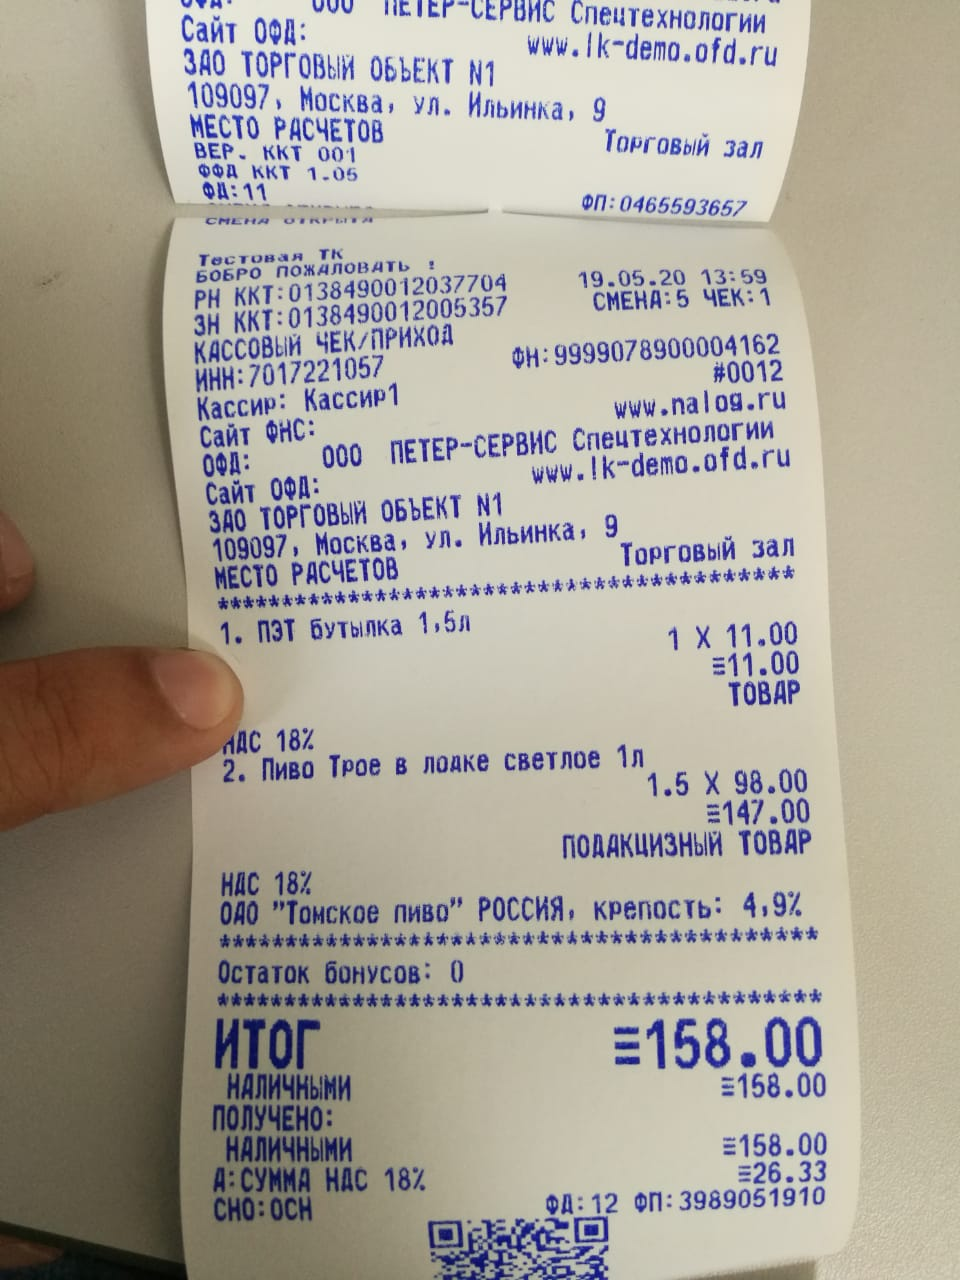
\includegraphics[width=125pt]{1.jpeg}} at (0pt,0pt)
   \end{tikzpicture}
   ;\par
   3. Поле <<СНО>> в чеке имеет значение <<ОСН>>;\par
   4. Второй чек вида:
   \begin{tikzpicture}
   \pgftext{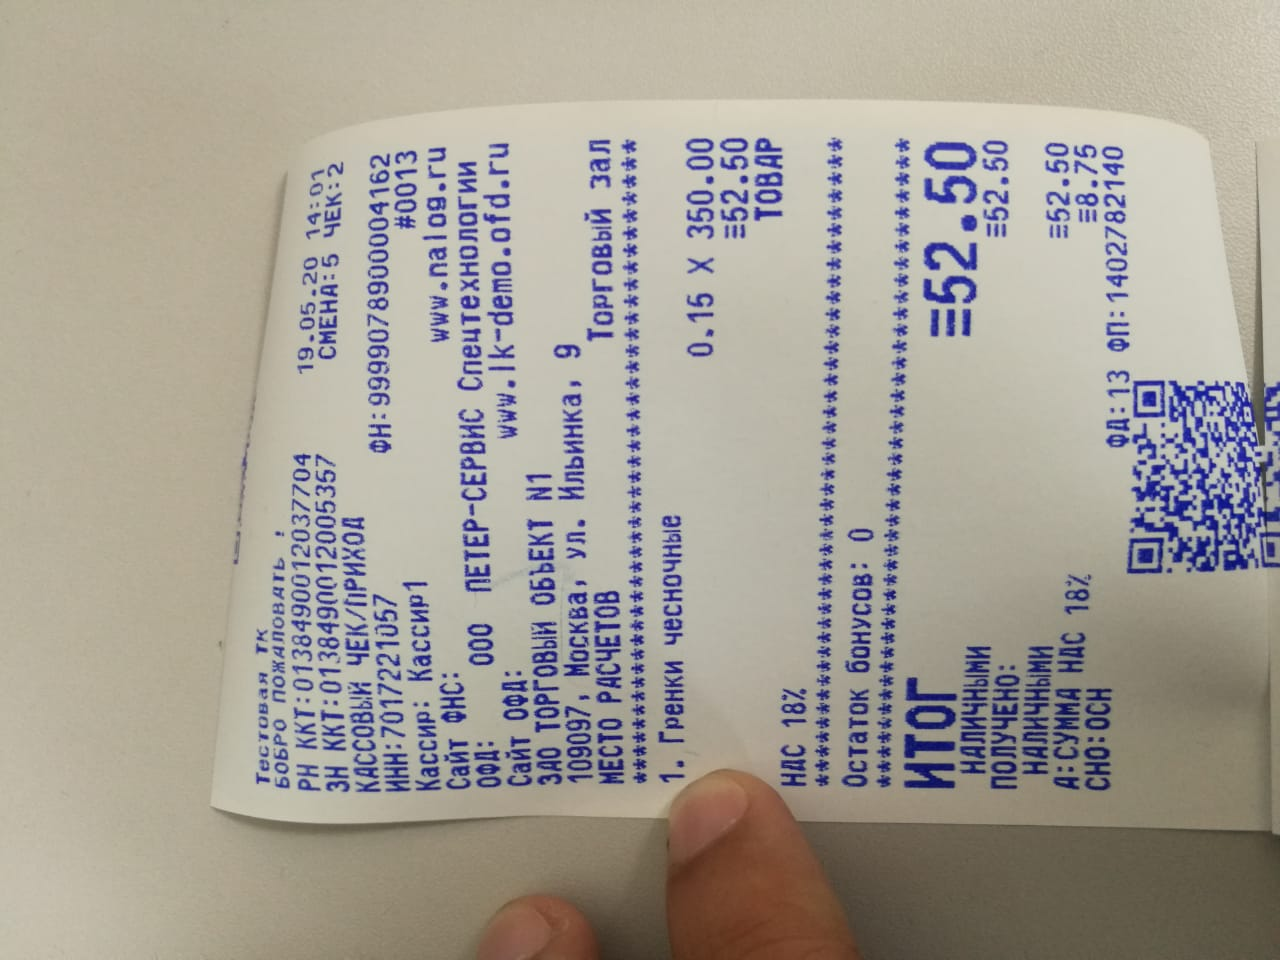
\includegraphics[width=125pt]{4.jpeg}} at (0pt,0pt)
   \end{tikzpicture}
   ;\par
   5. Поле <<СНО>> в чеке имеет значение <<УСН>>;\par
   6. Табличная часть <<Товары>> в форме рабочего места кассира очистится;\par
   &  \\
   \hline
   %****************************************************************************************************


   \multicolumn{4}{|c|}{\textbf{\textit{Проверка блокировки одновременной оплаты по безналичному расчету на разных кассах}}} \\
   \hline
   \hline
   \Rownum &  Проверить, что включена константа «крюВключитьБлокировкуПараллельнойОплатыЭквайринг» включить если не включена & Включена константа «крюВключитьБлокировкуПараллельнойОплатыЭквайринг» &  \\
   \hline
   \Rownum &  Проверить, что включена константа «крюБлокировкаПараллельнойОплатыЭквайринг» включить если не включена & Включена константа «крюБлокировкаПараллельнойОплатыЭквайринг» &
   \\
   \hline
   \Rownum & Запустить конфигурацию магазина выбрав пользователя <<Абрамовская Е. (кассир)>> & 1.Открылся общий интерфейс программы;\par
   2. Отображаются разделы <<Главное>> и <<Продажи>>;\par
   3. Открылась обработка <<Рабочее место кассира>>  &  \\
   \hline
   \Rownum	& Нажать кнопку \keys{Регистрация продаж} в меню РМК & 1. Форма меню РМК закрыта;\par
   2. Открыта форма с информационным сообщением для кассиров;\par
   3. Кнопка \keys{ОК} в нижней части формы недоступна &  \\
   \hline
   \Rownum	& Отметить чек бокс с надписью <<Мною прочитано и понято>> & 1. Чек бокс с надписью <<Мною прочитано и понято>> отмечен ;\par
   2. Кнопка \keys{ОК} в нижней части формы доступна &   \\
   \hline
   \Rownum	& Нажать кнопку \keys{ОК} в нижней части формы & 1. Форма с информационным сообщением для кассиров закрыта.;\par
   2. Открыта форма Рабочего места кассира  &  \\
   \hline
   \Rownum	& Нажать кнопку \keys{Поиск (F11)} в верхней части формы или горячую клавишу \keys{F11} & Открыта форма поиска и подбора товара в РМК &  \\
   \hline
   \Rownum	& Выбрать поиск по наименованию в выпадающем списке <<Поиск>> верхней части формы  & Выбран режим поиска по наименованию &  \\
   \hline
   \Rownum	& В поле поиска ввести <<Гренки чесночные>>  & В табличной части <<Товары>> осталась номенклатура, в наименовании которой содержится <<Гренки чесночные>> &  \\
   \hline
   \Rownum	& В табличной части <<Товары>> выбрать позицию с артикулом <<11432>>  & 1. Форма поиска закрылась;\par
   2. В табличную часть <<Товары>> формы рабочего места кассира добавлена позиция с артикулом <<11432>> с количеством <<1>> и установленной ценой &  \\
   \Rownum	& Установить количество позиции с артикулом <<11432>> равным <<0,150>>  & 1. Количество позиции с артикулом <<11432>> - <<Гренки чесночные>> изменилось на значение <<0,150>>&  \\
   \hline

   \Rownum	& Нажать кнопку \keys{Оплата (F8)} в верхней части формы или горячую клавишу \keys{F8}  &  Открыта форма оплаты &  \\
   \hline
   \Rownum	& Нажать кнопку \keys{Нал.(F6)} справа от поля ввода <<Всего к оплате (руб):>> или горячую клавишу \keys{F6}  & Появляется окно с сообщением <<"Осуществляется оплата по безналу на другой кассе, подождите...">> & !!!!!!!!!  \\
   \hline

   %****************************************************************************************************

     \multicolumn{4}{|c|}{\textbf{\textit{Проверка записи в регистре сведений <<крю Этапы пробития чека ККМ>>}}} \\
   \hline
   \hline
   \Rownum & Запустить конфигурацию магазина выбрав пользователя <<Абрамовская Е. (кассир)>> & 1.Открылся общий интерфейс программы;\par
   2. Отображаются разделы <<Главное>> и <<Продажи>>;\par
   3. Открылась обработка <<Рабочее место кассира>>  &  \\
   \hline
   \Rownum	& Нажать кнопку \keys{Регистрация продаж} в меню РМК & 1. Форма меню РМК закрыта;\par
   2. Открыта форма с информационным сообщением для кассиров;\par
   3. Кнопка \keys{ОК} в нижней части формы недоступна &  \\
   \hline
   \Rownum	& Отметить чек бокс с надписью <<Мною прочитано и понято>> & 1. Чек бокс с надписью <<Мною прочитано и понято>> отмечен ;\par
   2. Кнопка \keys{ОК} в нижней части формы доступна &   \\
   \hline
   \Rownum	& Нажать кнопку \keys{ОК} в нижней части формы & 1. Форма с информационным сообщением для кассиров закрыта.;\par
   2. Открыта форма Рабочего места кассира  &  \\
   \hline
   \Rownum	& Нажать кнопку \keys{Поиск (F11)} в верхней части формы или горячую клавишу \keys{F11} & Открыта форма поиска и подбора товара в РМК &  \\
   \hline
   \Rownum	& Выбрать поиск по наименованию в выпадающем списке <<Поиск>> верхней части формы  & Выбран режим поиска по наименованию &  \\
   \hline
   \Rownum	& В поле поиска ввести <<Трое в лодке светлое>>  & В табличной части <<Товары>> осталась номенклатура, в наименовании которой содержится <<Трое в лодке светлое>> &  \\
   \hline
   \Rownum	& В табличной части <<Товары>> выбрать позицию с артикулом <<11697>>  & 1. Форма поиска закрылась;\par
   2. В табличную часть <<Товары>> формы рабочего места кассира добавлена позиция с артикулом <<11697>> с количеством <<1>> и установленной ценой &  \\
   \hline
   \Rownum	& Нажать кнопку \keys{Поиск (F11)} в верхней части формы или горячую клавишу \keys{F11} & Открыта форма поиска и подбора товара в РМК &  \\
   \hline
   \Rownum	& Выбрать поиск по наименованию в выпадающем списке <<Поиск>> верхней части формы  & Выбран режим поиска по наименованию &  \\
   \hline
   \Rownum	& В поле поиска ввести <<Пакет Крюгер Хаус маленький>>  & В табличной части <<Товары>> осталась номенклатура, в наименовании которой содержится <<Пакет Крюгер Хаус маленький>> &  \\
   \hline
   \Rownum	& В табличной части <<Товары>> выбрать позицию с артикулом <<10347>>  & 1. Форма поиска закрылась;\par
   2. В табличную часть <<Товары>> формы рабочего места кассира добавлена позиция с артикулом <<10347>> с количеством <<1>> и установленной ценой &  \\
   \hline
   \Rownum	& Нажать \keys{Ctrl} + \keys{M}   & 1. В табличную часть <<Товары>> формы рабочего места кассира добавлена позиция с артикулом <<10340>> - <<ПЭТ бутылка 1,5л>>  &  \\
   \hline
   \Rownum	& Установить количество позиции с артикулом <<10340>> равным <<1>>  & 1. Количество позиции с артикулом <<11697>> - <<Пиво Трое в лодке светлое 1л>> изменилось на значение <<1.5>>&  \\
   \hline
   \Rownum	& Нажать кнопку \keys{Оплата (F8)} в верхней части формы или горячую клавишу \keys{F8}  &  Открыта форма оплаты &  \\
   \hline
   \Rownum	& Нажать кнопку \keys{Нал.(F6)} справа от поля ввода <<Всего к оплате (руб):>> или горячую клавишу \keys{F6}  & В табличную часть <<Виды оплат>> добавлена строка со значениями полей: <<Вида оплаты>> - <<Наличные>>; <<Сумма>> - рассчитанной суммой&  \\
   \hline
   \Rownum	& Нажать кнопку \keys{Enter} в области цифровых кнопок или горячую клавишу \keys{Ctrl + Enter}  & 1. Форма оплаты закроется;\par
   2. Табличная часть <<Товары>> в форме рабочего места кассира очистится&  \\
   \hline
   \Rownum & Закрыть рабочее место кассира нажав последовательно горячие клавиши \keys{F10} - \keys{F12}  & Открылось меню <<Рабочего места кассира>> &  \\
   \hline
   \Rownum & Нажать кнопку \keys{Завершение работы}   & Конфигурация закрылась
   &  \\
   \hline
   \Rownum & Запустить конфигурацию магазина  & 1.Открылся общий интерфейс программы;\par
   2. Отображаются все доступные разделы  &  \\
   \hline
   \Rownum & Перейти в раздел <<Продажи>>   & 1. Открылся отдел <<Продажи>>
   &  \\
    \hline
   \Rownum	& Выбрать пункт  <<Чеки>> & Открылся форма списка документов <<Чек ККМ>> &  \\
   &  \\
   \hline
   \Rownum & Выбрать последний созданный чек, открыть его  & Открылся форма  документа <<Чек ККМ>> &  \\
   &  \\
    \hline
   \Rownum & Перейти на вкладку <<Комментарий>>  & 1. Открылась вкладка <<Комментарий>>;\par
   2. Табличная часть под полем <<Комментарий>>, заполнена данными из регистра сведений <<крю Этапы пробития чека ККМ>> относящимися к текущему чеку  &  \\
   &  \\
   \hline
   %****************************************************************************************************


    \multicolumn{4}{|c|}{\textbf{\textit{В форме меню, если есть необработанные чеки блокируются все элементы кроме <<Регистрации продаж>> и сообщение разобраться с ошибками чеков}}} \\
    \hline
    \hline
   \Rownum & Запустить конфигурацию магазина выбрав пользователя <<Абрамовская Е. (кассир)>> & 1.Открылся общий интерфейс программы;\par
   2. Отображаются разделы <<Главное>> и <<Продажи>>;\par
   3. Открылась обработка <<Рабочее место кассира>>  &  \\
   \hline
   \Rownum	& Нажать кнопку \keys{Регистрация продаж} в меню РМК & 1. Форма меню РМК закрыта;\par
   2. Открыта форма с информационным сообщением для кассиров;\par
   3. Кнопка \keys{ОК} в нижней части формы недоступна &  \\
   \hline
   \Rownum	& Отметить чек бокс с надписью <<Мною прочитано и понято>> & 1. Чек бокс с надписью <<Мною прочитано и понято>> отмечен ;\par
   2. Кнопка \keys{ОК} в нижней части формы доступна &   \\
   \hline
   \Rownum	& Нажать кнопку \keys{ОК} в нижней части формы & 1. Форма с информационным сообщением для кассиров закрыта.;\par
   2. Открыта форма Рабочего места кассира  &  \\
   \hline
   \Rownum	& Нажать кнопку \keys{Поиск (F11)} в верхней части формы или горячую клавишу \keys{F11} & Открыта форма поиска и подбора товара в РМК &  \\
   \hline
   \Rownum	& Выбрать поиск по наименованию в выпадающем списке <<Поиск>> верхней части формы  & Выбран режим поиска по наименованию &  \\
   \hline
   \Rownum	& В поле поиска ввести <<Трое в лодке светлое>>  & В табличной части <<Товары>> осталась номенклатура, в наименовании которой содержится <<Трое в лодке светлое>> &  \\
   \hline
   \Rownum	& В табличной части <<Товары>> выбрать позицию с артикулом <<11697>>  & 1. Форма поиска закрылась;\par
   2. В табличную часть <<Товары>> формы рабочего места кассира добавлена позиция с артикулом <<11697>> с количеством <<1>> и установленной ценой &  \\
   \hline
   \Rownum	& Нажать кнопку \keys{Поиск (F11)} в верхней части формы или горячую клавишу \keys{F11} & Открыта форма поиска и подбора товара в РМК &  \\
   \hline
   \Rownum	& Выбрать поиск по наименованию в выпадающем списке <<Поиск>> верхней части формы  & Выбран режим поиска по наименованию &  \\
   \hline
   \Rownum	& В поле поиска ввести <<Пакет Крюгер Хаус маленький>>  & В табличной части <<Товары>> осталась номенклатура, в наименовании которой содержится <<Пакет Крюгер Хаус маленький>> &  \\
   \hline
   \Rownum	& В табличной части <<Товары>> выбрать позицию с артикулом <<10347>>  & 1. Форма поиска закрылась;\par
   2. В табличную часть <<Товары>> формы рабочего места кассира добавлена позиция с артикулом <<10347>> с количеством <<1>> и установленной ценой &  \\
   \hline
   \Rownum	& Нажать \keys{Ctrl} + \keys{M}   & 1. В табличную часть <<Товары>> формы рабочего места кассира добавлена позиция с артикулом <<10340>> - <<ПЭТ бутылка 1,5л>>  &  \\
   \hline
   \Rownum	& Установить количество позиции с артикулом <<10340>> равным <<1>>  & 1. Количество позиции с артикулом <<11697>> - <<Пиво Трое в лодке светлое 1л>> изменилось на значение <<1.5>>&  \\
   \hline
   \Rownum	& Нажать кнопку \keys{Оплата (F8)} в верхней части формы или горячую клавишу \keys{F8}  &  Открыта форма оплаты &  \\
   \hline
   \Rownum	& Нажать кнопку \keys{Нал.(F6)} справа от поля ввода <<Всего к оплате (руб):>> или горячую клавишу \keys{F6}  & В табличную часть <<Виды оплат>> добавлена строка со значениями полей: <<Вида оплаты>> - <<Наличные>>; <<Сумма>> - рассчитанной суммой&  \\
   \hline
   \Rownum	& Нажать кнопку \keys{Enter} в области цифровых кнопок или горячую клавишу \keys{Ctrl + Enter} Передварительно связавшись с представителем заказчика, для отключения питания фискального регистратора в моментпробития чека, что бы инициировать ошибочную ситуацию  & 1. Форма оплаты закроется;\par
   2. Табличная часть <<Товары>> в форме рабочего места кассира очистится&  \\
   \hline

   \Rownum & Закрыть рабочее место кассира нажав последовательно горячие клавиши \keys{F10} - \keys{F12}  &1.  Открылось меню <<Рабочего места кассира>>;\par
   2. В меню доступны только кнопки: \keys{Регистрация продаж}, \keys{Закрыть}, \keys{Завершение работы}   &  \\
   \hline
   \Rownum & Нажать кнопку \keys{Завершение работы}   & Конфигурация закрылась
   &  \\
    \hline
   \Rownum & Запустить конфигурацию магазина выбрав пользователя <<Абрамовская Е. (кассир)>> & 1.Открылся общий интерфейс программы;\par
   2. Отображаются разделы <<Главное>> и <<Продажи>>;\par
   3. Открылась обработка <<Рабочее место кассира>> ;\par
   4. Открылась форма <<Ошибка непроведенных чеков>> с сообщением об ошибке <<Есть не обработанные чеки ККМ. Необходимо зайти «Регистрация продаж» -> Кнопка «Проверить Чеки ККМ» и проанализировать почему чек не пробит>> &  \\
   \hline

   \Rownum & Нажать кнопку \keys{Закрыть} на форме с описанием ошибки  & Форма с описанием ошибки закрылась
   &  \\
   \hline
    \Rownum & Нажать кнопку \keys{Завершение работы}   & Конфигурация закрылась
   &  \\
   \hline
    %****************************************************************************************************

     \multicolumn{4}{|c|}{\textbf{\textit{При возникновении ошибок прежде чем пробивать новый чек, необходимо закончить работу со старым}}} \\
    \hline
    \hline
       \Rownum & Запустить конфигурацию магазина выбрав пользователя <<Абрамовская Е. (кассир)>> & 1.Открылся общий интерфейс программы;\par
    2. Отображаются разделы <<Главное>> и <<Продажи>>;\par
    3. Открылась обработка <<Рабочее место кассира>> ;\par
    4. Открылась форма <<Ошибка непроведенных чеков>> с сообщением об ошибке <<Есть не обработанные чеки ККМ. Необходимо зайти «Регистрация продаж» -> Кнопка «Проверить Чеки ККМ» и проанализировать почему чек не пробит>> &  \\
    \hline
    \Rownum & Нажать кнопку \keys{Закрыть} на форме с описанием ошибки  & Форма с описанием ошибки закрылась
    &  \\
    \hline
    \Rownum	& Нажать кнопку \keys{Регистрация продаж} в меню РМК & 1. Форма меню РМК закрыта;\par
    2. Открыта форма с информационным сообщением для кассиров;\par
    3. Кнопка \keys{ОК} в нижней части формы недоступна &  \\
    \hline
    \Rownum	& Отметить чек бокс с надписью <<Мною прочитано и понято>> & 1. Чек бокс с надписью <<Мною прочитано и понято>> отмечен ;\par
    2. Кнопка \keys{ОК} в нижней части формы доступна &   \\
    \hline
    \Rownum	& Нажать кнопку \keys{ОК} в нижней части формы & 1. Форма с информационным сообщением для кассиров закрыта.;\par
    2. Открыта форма Рабочего места кассира  &  \\
    \hline
    \Rownum	& Нажать кнопку \keys{Поиск (F11)} в верхней части формы или горячую клавишу \keys{F11} & Открыта форма поиска и подбора товара в РМК &  \\
    \hline
    \Rownum	& Выбрать поиск по наименованию в выпадающем списке <<Поиск>> верхней части формы  & Выбран режим поиска по наименованию &  \\
    \hline
    \Rownum	& В поле поиска ввести <<Трое в лодке светлое>>  & В табличной части <<Товары>> осталась номенклатура, в наименовании которой содержится <<Трое в лодке светлое>> &  \\
    \hline
    \Rownum	& В табличной части <<Товары>> выбрать позицию с артикулом <<11697>>  & 1. Форма поиска закрылась;\par
    2. Под табличной частью <<Товары>> появилось сообщение об ошибке содержащее номер чека, вид оплаты и сообщением <<Для дальнейшей работы на данной кассе требуется устранить указанную проблему!>>, ниже выводится еще одно сообщение <<Нажмите кнопку «Проверить Чеки ККМ»>>
    &  \\
    \hline
    \Rownum	& Закрыть сообщение об ошибке & 1. Сообщение об ошибке закрылось;\par
    2. Табличная часть <<Товары>> не содержит строк. &  \\
    \hline

    \Rownum & Закрыть рабочее место кассира нажав последовательно горячие клавиши \keys{F10} - \keys{F12}  &1.  Открылось меню <<Рабочего места кассира>>;\par
    2. В меню доступны только кнопки: \keys{Регистрация продаж}, \keys{Закрыть}, \keys{Завершение работы}   &  \\
    \hline
    \Rownum & Нажать кнопку \keys{Завершение работы}   & Конфигурация закрылась
    &  \\
    \hline
    %****************************************************************************************************



    \multicolumn{4}{|c|}{\textbf{\textit{Тестирование алгоритма проверки чеков ККМ}}} \\
    \hline
    \hline
    \Rownum & Запустить конфигурацию магазина выбрав пользователя <<Абрамовская Е. (кассир)>> & 1.Открылся общий интерфейс программы;\par
    2. Отображаются разделы <<Главное>> и <<Продажи>>;\par
    3. Открылась обработка <<Рабочее место кассира>> ;\par
    4. Открылась форма <<Ошибка непроведенных чеков>> с сообщением об ошибке <<Есть не обработанные чеки ККМ. Необходимо зайти «Регистрация продаж» -> Кнопка «Проверить Чеки ККМ» и проанализировать почему чек не пробит>> &  \\
    \hline
    \Rownum & Нажать кнопку \keys{Закрыть} на форме с описанием ошибки  & Форма с описанием ошибки закрылась
    &  \\
    \hline
    \Rownum	& Нажать кнопку \keys{Регистрация продаж} в меню РМК & 1. Форма меню РМК закрыта;\par
    2. Открыта форма с информационным сообщением для кассиров;\par
    3. Кнопка \keys{ОК} в нижней части формы недоступна &  \\
    \hline
    \Rownum	& Отметить чек бокс с надписью <<Мною прочитано и понято>> & 1. Чек бокс с надписью <<Мною прочитано и понято>> отмечен ;\par
    2. Кнопка \keys{ОК} в нижней части формы доступна &   \\
    \hline
    \Rownum	& Нажать кнопку \keys{ОК} в нижней части формы & 1. Форма с информационным сообщением для кассиров закрыта.;\par
    2. Открыта форма Рабочего места кассира  &  \\
    \hline
    \Rownum	& Нажать кнопку \keys{Проверить чеки ККМ} в верхней части формы  &1.  Открыта форма <<Проверка чека ККМ>>;\par
    2. В табличной части формы содержатся две строки с номерами чеков в первой колонке  и описанием проблемы: <<Наличная оплата. Фискальный чек возможно был распечатан. Проверка будет выполнена после нажатия на кнопку «Распечатать фискальный чек». При необходимости чек будет распечатан.>> во второй;\par
    3. Внизу формы в окне сообщений отображаются две строки с текстом <<В первую очередь должен быть обработан ---> Чек>> и номером чека &  \\
    \hline
    \Rownum	& Закрыть окно сообщений  & Окно сообщений закрыто &  \\
    \hline
    \Rownum	& В табличной части выделить строку содержащую чек с номером, который был указан в строке сообщений  & В табличной части Выделена строка с чеком &  \\
    \hline
    \Rownum	& Нажать кнопку \keys{Распечатать фискальный чек}, кнопка с изображением фискального регистратора, справа от табличной части, третья сверху.  & 1. Фискальный регистратор распечатал текущий чек;\par
    2. В табличной части отсталась одна выделенная строка с чеком &  \\
    \hline
    \Rownum	& Нажать кнопку \keys{Команда выбрать}, кнопка с изображением зеленого треугольника, справа от табличной части, четвертая сверху. или горячую клавишу \keys{Ctrl + Enter}   & Открылась форма текущего чека  &  \\
    \hline
    \Rownum	& Закрыть форму текущего чека либо просто закрыв форму, либо нажав кнопку \keys{Провести и закрыть}  & Форма чека закрылась&  \\
    \hline
    \Rownum	& Нажать кнопку \keys{Распечатать фискальный чек}, кнопка с изображением фискального регистратора, справа от табличной части, третья сверху.  & 1. Фискальный регистратор распечатал текущий чек;\par
    2. Табличная часть очистилась &  \\
    \hline
    \Rownum	& Закрыть форму <<Проверка чека ККМ>> &  Форма <<Проверка чека ККМ>> закрыта &  \\
    \hline


    \Rownum & Закрыть рабочее место кассира нажав последовательно горячие клавиши \keys{F10} - \keys{F12}  &1.  Открылось меню <<Рабочего места кассира>>;\par
    2. В меню доступны все кнопки   &  \\
    \hline
    \Rownum & Нажать кнопку \keys{Завершение работы}   & Конфигурация закрылась
    &  \\
    \hline
    %****************************************************************************************************


    \multicolumn{4}{|c|}{\textbf{\textit{Алгоритм фиксации времени прохождения этапов набора, проведения и пробития чека}}} \\
    \hline
    \hline
     \Rownum & Запустить конфигурацию магазина выбрав пользователя <<Абрамовская Е. (кассир)>> & 1.Открылся общий интерфейс программы;\par
   2. Отображаются разделы <<Главное>> и <<Продажи>>;\par
   3. Открылась обработка <<Рабочее место кассира>>  &  \\
   \hline
   \Rownum	& Нажать кнопку \keys{Регистрация продаж} в меню РМК & 1. Форма меню РМК закрыта;\par
   2. Открыта форма с информационным сообщением для кассиров;\par
   3. Кнопка \keys{ОК} в нижней части формы недоступна &  \\
   \hline
   \Rownum	& Отметить чек бокс с надписью <<Мною прочитано и понято>> & 1. Чек бокс с надписью <<Мною прочитано и понято>> отмечен ;\par
   2. Кнопка \keys{ОК} в нижней части формы доступна &   \\
   \hline
   \Rownum	& Нажать кнопку \keys{ОК} в нижней части формы & 1. Форма с информационным сообщением для кассиров закрыта.;\par
   2. Открыта форма Рабочего места кассира  &  \\
   \hline
   \Rownum	& Нажать кнопку \keys{Поиск (F11)} в верхней части формы или горячую клавишу \keys{F11} & Открыта форма поиска и подбора товара в РМК &  \\
   \hline
   \Rownum	& Выбрать поиск по наименованию в выпадающем списке <<Поиск>> верхней части формы  & Выбран режим поиска по наименованию &  \\
   \hline
   \Rownum	& В поле поиска ввести <<Трое в лодке светлое>>  & В табличной части <<Товары>> осталась номенклатура, в наименовании которой содержится <<Трое в лодке светлое>> &  \\
   \hline
   \Rownum	& В табличной части <<Товары>> выбрать позицию с артикулом <<11697>>  & 1. Форма поиска закрылась;\par
   2. В табличную часть <<Товары>> формы рабочего места кассира добавлена позиция с артикулом <<11697>> с количеством <<1>> и установленной ценой &  \\
   \hline
   \Rownum	& Нажать кнопку \keys{Поиск (F11)} в верхней части формы или горячую клавишу \keys{F11} & Открыта форма поиска и подбора товара в РМК &  \\
   \hline
   \Rownum	& Выбрать поиск по наименованию в выпадающем списке <<Поиск>> верхней части формы  & Выбран режим поиска по наименованию &  \\
   \hline
   \Rownum	& В поле поиска ввести <<Пакет Крюгер Хаус маленький>>  & В табличной части <<Товары>> осталась номенклатура, в наименовании которой содержится <<Пакет Крюгер Хаус маленький>> &  \\
   \hline
   \Rownum	& В табличной части <<Товары>> выбрать позицию с артикулом <<10347>>  & 1. Форма поиска закрылась;\par
   2. В табличную часть <<Товары>> формы рабочего места кассира добавлена позиция с артикулом <<10347>> с количеством <<1>> и установленной ценой &  \\
   \hline
   \Rownum	& Нажать \keys{Ctrl} + \keys{M}   & 1. В табличную часть <<Товары>> формы рабочего места кассира добавлена позиция с артикулом <<10340>> - <<ПЭТ бутылка 1,5л>>  &  \\
   \hline
   \Rownum	& Установить количество позиции с артикулом <<10340>> равным <<1>>  & 1. Количество позиции с артикулом <<11697>> - <<Пиво Трое в лодке светлое 1л>> изменилось на значение <<1.5>>&  \\
   \hline
   \Rownum	& Нажать кнопку \keys{Оплата (F8)} в верхней части формы или горячую клавишу \keys{F8}  &  Открыта форма оплаты &  \\
   \hline
   \Rownum	& Нажать кнопку \keys{Нал.(F6)} справа от поля ввода <<Всего к оплате (руб):>> или горячую клавишу \keys{F6}  & В табличную часть <<Виды оплат>> добавлена строка со значениями полей: <<Вида оплаты>> - <<Наличные>>; <<Сумма>> - рассчитанной суммой&  \\
   \hline
   \Rownum	& Нажать кнопку \keys{Enter} в области цифровых кнопок или горячую клавишу \keys{Ctrl + Enter}  & 1. Форма оплаты закроется;\par
   2. На фискальном регистраторе будет напечатан чек  ;\par
   3. Табличная часть <<Товары>> в форме рабочего места кассира очистится
   &  \\
   \hline
   \Rownum & Закрыть рабочее место кассира нажав последовательно горячие клавиши \keys{F10} - \keys{F12}  &1.  Открылось меню <<Рабочего места кассира>>;\par
   2. В меню доступны все кнопки   &  \\
   \hline
   \Rownum & Нажать кнопку \keys{Завершение работы}   & Конфигурация закрылась
   &  \\
   \hline
    \Rownum & Запустить конфигурацию магазина  & 1.Открылся общий интерфейс программы;\par
   2. Отображаются все доступные разделы  &  \\
   \hline
   \Rownum &   Перейти в раздел <<Продажи>>   & 1. Открылся отдел <<Продажи>>
   &  \\

   \hline
   \Rownum	& Выбрать пункт <<Дополнительные отчеты>>  & Открылся форма выбора дополнительных отчетов <<Дополнительные отчеты (Продажи)>>   &  \\
   \hline
   \Rownum	& Выбрать отчет <<Замеры времени пробития чеков>>, если он отсутствует в списке, добавить используя пункт <<Настроить список>> в левом нижнем углу формы & Открылась форма отчета <<Замеры времени пробития чеков>>   &  \\
   \hline
   \Rownum	& Нажать кнопку \keys{Сформировать}  & 1. Отчет  <<Замеры времени пробития чеков>> сформирован;\par
   2. В отчете присутствует последний пробитый чек  и данные замеров по этому чеку  &  \\
   \hline
   \Rownum	& Закрыть отчет  & Форма отчета закрыта  &  \\
   \hline
   \Rownum	& Закрыть конфигурацию  & Конфигурация закрыта  &  \\
   \hline
    %****************************************************************************************************




     \multicolumn{4}{|c|}{\textbf{\textit{Проверка блокировки возврата покупателю при сложных чеках и оплате по безналичному расчету}}} \\
    \hline
    \hline
    \Rownum & Запустить конфигурацию магазина выбрав пользователя <<Абрамовская Е. (кассир)>> & 1.Открылся общий интерфейс программы;\par
    2. Отображаются разделы <<Главное>> и <<Продажи>>;\par
    3. Открылась обработка <<Рабочее место кассира>>  &  \\
    \hline
    \Rownum	& Нажать кнопку \keys{Регистрация продаж} в меню РМК & 1. Форма меню РМК закрыта;\par
    2. Открыта форма с информационным сообщением для кассиров;\par
    3. Кнопка \keys{ОК} в нижней части формы недоступна &  \\
    \hline
    \Rownum	& Отметить чек бокс с надписью <<Мною прочитано и понято>> & 1. Чек бокс с надписью <<Мною прочитано и понято>> отмечен ;\par
    2. Кнопка \keys{ОК} в нижней части формы доступна &   \\
    \hline
    \Rownum	& Нажать кнопку \keys{ОК} в нижней части формы & 1. Форма с информационным сообщением для кассиров закрыта.;\par
    2. Открыта форма Рабочего места кассира  &  \\
    \hline
    \Rownum	& Нажать кнопку \keys{Поиск (F11)} в верхней части формы или горячую клавишу \keys{F11} & Открыта форма поиска и подбора товара в РМК &  \\
    \hline
    \Rownum	& Выбрать поиск по наименованию в выпадающем списке <<Поиск>> верхней части формы  & Выбран режим поиска по наименованию &  \\
    \hline
    \Rownum	& В поле поиска ввести <<Гренки чесночные>>  & В табличной части <<Товары>> осталась номенклатура, в наименовании которой содержится <<Гренки чесночные>> &  \\
    \hline
    \Rownum	& В табличной части <<Товары>> выбрать позицию с артикулом <<11432>>  & 1. Форма поиска закрылась;\par
    2. В табличную часть <<Товары>> формы рабочего места кассира добавлена позиция с артикулом <<11432>> с количеством <<1>> и установленной ценой &  \\
    \Rownum	& Установить количество позиции с артикулом <<11432>> равным <<0,150>>  & 1. Количество позиции с артикулом <<11432>> - <<Гренки чесночные>> изменилось на значение <<0,150>>&  \\
    \hline
    \Rownum	& Нажать кнопку \keys{Поиск (F11)} в верхней части формы или горячую клавишу \keys{F11} & Открыта форма поиска и подбора товара в РМК &  \\
    \hline
    \Rownum	& Выбрать поиск по наименованию в выпадающем списке <<Поиск>> верхней части формы  & Выбран режим поиска по наименованию &  \\
    \hline
    \Rownum	& В поле поиска ввести <<Трое в лодке светлое>>  & В табличной части <<Товары>> осталась номенклатура, в наименовании которой содержится <<Трое в лодке светлое>> &  \\
    \hline
    \Rownum	& В табличной части <<Товары>> выбрать позицию с артикулом <<11697>>  & 1. Форма поиска закрылась;\par
    2. В табличную часть <<Товары>> формы рабочего места кассира добавлена позиция с артикулом <<11697>> с количеством <<1>> и установленной ценой &  \\
    \hline
    \Rownum	& Нажать \keys{Ctrl} + \keys{M}   & 1. В табличную часть <<Товары>> формы рабочего места кассира добавлена позиция с артикулом <<10340>> - <<ПЭТ бутылка 1,5л>>  &  \\
    \hline
    \Rownum	& Установить количество позиции с артикулом <<10340>> равным <<1>>  & 1. Количество позиции с артикулом <<11697>> - <<Пиво Трое в лодке светлое 1л>> изменилось на значение <<1.5>>&  \\
    \hline
    \Rownum	& Нажать кнопку \keys{Оплата (F8)} в верхней части формы или горячую клавишу \keys{F8}  &  Открыта форма оплаты &  \\
    \hline
    \Rownum	& Нажать кнопку \keys{ПК.(F7)} справа от поля ввода <<Всего к оплате (руб):>> или горячую клавишу \keys{F7}  & В табличную часть <<Виды оплат>> добавлена строка со значениями полей: <<Вида оплаты>> - <<Оплата картой>>; <<Сумма>> - рассчитанной суммой&  \\
    \hline
    \Rownum	& После предложения вставить карту, обратитсяя к сотруднику заказчика для осуществления оплаты картой  & Оплата картой произведена&  \\
    \hline
     \Rownum	& Нажать кнопку \keys{Enter} в области цифровых кнопок или горячую клавишу \keys{Ctrl + Enter}  & 1. Форма оплаты закроется;\par
    2. На фискальном регистраторе будет напечатан чек;\par
    3. Табличная часть <<Товары>> в форме рабочего места кассира очистится &  \\
    \hline
    \Rownum	& Нажать кнопку \keys{Возврат (F5)} в области цифровых кнопок или горячую клавишу \keys{F5}  & 1. Открылась форма возврата чека;\par
    2. В верхней части формы поля <<С:>> и <<По:>> в качестве значения имеют текущую дату;\par
    3. Табличная часть <<Товары>> в форме рабочего места кассира очистится &  \\
    \hline
    \Rownum	& В табличной части выбрать первую строку  & Выбрана первая строка &  \\
    \hline
    \Rownum	& Нажать кнопку \keys{Команда выбрать}, кнопка с изображением зеленого треугольника, справа от табличной части, первая сверху. или горячую клавишу \keys{Ctrl + Enter}   & Открылась форма <<Возврат недоступен>> с текстом ошибки: <<"Корректный возврат разбитого чека по кулинарии, с видом оплаты «Оплата картой», невозможен.  Выполните возврат наличными деньгами>> &  \\
    \hline
    \Rownum	& Закрыть форму с сообщением об ошибке  & Форма с сообщением об ошибке закрыта &  \\
    \hline
    \Rownum & Закрыть рабочее место кассира нажав последовательно горячие клавиши \keys{F10} - \keys{F12}  &1.  Открылось меню <<Рабочего места кассира>>;\par
    2. В меню доступны все кнопки   &  \\
    \hline
    \Rownum & Нажать кнопку \keys{Завершение работы}   & Конфигурация закрылась
    &  \\
    \hline
    %****************************************************************************************************

   %****************************************************************************************************

\end{longtable}



